%*** Muon system momentum resolution parameterization
%\documentstyle[epsf]{article}
%\documentstyle[sgmlext,epsf,cernart,12pt]{article}


\documentclass[epsf]{article}

%**************************** General libraries *******************************
\usepackage{graphicx}
\usepackage{epsf}
\usepackage{pdfpages}

\usepackage{mathtools}
\usepackage{cancel}
\usepackage[utf8]{inputenc} 
\usepackage{amssymb}
\usepackage{ntheorem}
\usepackage{tensor}
%\usepackage{physics}
\usepackage[italicdiff]{physics}
\usepackage{calc}
\usepackage{caption}
%\usepackage{subcaption}
\usepackage{tcolorbox}
\usepackage{chngcntr}
\usepackage{titlesec}
\usepackage {graphicx,float} 
\usepackage{subfig}
\usepackage{siunitx}
\usepackage{xcolor}
\usepackage{etoolbox} %ifthen
\usepackage[outline]{contour} % glow around text

%\renewcommand{\pt}{\mbox{$p_{t}$}\ }
\def\be{\begin{equation}}
\def\ee{\end{equation}}
%\def\sqrtkgy{\sqrt{m^2-\nabla^2_y}}
\def\btopipi{\rm B \rightarrow \pi^+\pi^-}
%\input epsf
\topmargin=10mm
\textheight=215mm
\textwidth=160mm
\pagenumbering{arabic}
\pagestyle{plain}
\baselineskip 25pt
\begin{document}
\baselineskip 25pt
\begin{titlepage}
\baselineskip 25pt
%\docnum{UCD-IIRPA-97-28}
\date{}
\title{A Monte Carlo Study of the Relativistic
Harmonic Oscillator\footnote{This 
research was supported in part by the U.S. Department
of Energy: DE-FG03-91ER40674.} }
\author{John R. Smith\footnote{Corresponding author: Tel: +1 530.752.3062; 
Fax: +1 530.752.2431; e-mail: jrsmith@ucdavis.edu} 
and Stephen P. Smith\footnote{UC Davis Visiting Scientist}  \\
{\em University of California, Davis}\\
{\em Davis, California 95616-8677\ USA}}
\abstract{Abstract}
\baselineskip 25pt
\pagenumbering{arabic}
We present a Monte Carlo calculation of the ground-state
wave function for the relativistic harmonic oscillator using the 
classical action in the path integral representation of quantum mechanics.
The ground-state wave function has the usual Gaussian shape in the 
non-relativistic limit, but is not described by a single Gaussian 
function in the extreme relativistic limit and appears to remain 
square-integrable for arbitrary values of $mc^2/\hbar\omega$.
A comparison is made with the ground state of the Klein-Gordon
equation in the presence of the harmonic oscillator potential and
the differences are presented.
Also we present a realization of the non-relativistic 
ground-state problem in terms
of a first-order auto-regressive time series with an extension for
periodicity which can be 
implemented as a $3n$ computer algorithm.
\vskip 0.5 truein
\centerline{PACS numbers: 03.65.-w;\quad 03.65.Pm;\quad 03.65.Ge;
\quad 03.30.+p}
%\tableofcontents
%\listoffigures
\end{titlepage}
%
\section{Introduction }
The theory of elementary sca\-lar particles is of central importance 
for the Standard Model because of the Higgs mechanism. In addition
there have been many attempts to calculate relativistic bound states 
based on the harmonic oscillator potential and other confinement
mechanisms \cite{bib:gunion1}, \cite{bib:gunion2}, \cite{bib:hey}.
Even though the harmonic oscillator potential is used 
in the context of the Klein-Gordon equation 
for the above bound-state calculations we
should keep in mind that the propagation and interaction of 
elementary sca\-lar particles such as the 
Higgs boson is ultimately an experimental question which may lead to 
modifications of the current quantum mechanical theory of such particles.

In this paper we take a close look at two different methods to 
make quantum mechanical calculations and compare their results for
scalar particles interacting with a simple harmonic oscillator potential.
The usual picture used in these computations 
is based on the Klein-Gordon equation which makes a definite choice of the 
representation for momentum and position operators. An alternative viewpoint
is to use the Feynman path integral. 
The classical relativistic action deviates sufficiently from 
the polynomial form used in Klein-Gordon case that 
a direct comparison of the two approaches is worthwhile.
Both methods agree in the non-relativistic limit, but this letter shows
that there are significant differences in the relativistic regime.

We use the classical action instead of the classical Hamiltonian because we
want investigate the implications of 
using the original Feynman correspondence principle.
According to the 
Feynman correspondence principle the classical path is the only path to 
contribute to the path integral involving the classical action 
as $\hbar \rightarrow 0$. The Feynman correspondence principle, 
therefore, differs somewhat from 
the Bohr-Dirac correspondence principle which holds $\hbar$ finite and 
demonstrates that quantum mechanics 
goes over to classical mechanics in the limit of large quantum numbers.

We make no assumptions about operators or commutation relations and 
instead use a Monte Carlo
method based on the Metropolis algorithm \cite{bib:metropolis} with 
a Euclidean metric 
to investigate the ground state of the relativistic harmonic oscillator.
We then present a comparison with the ground state computed from the
Klein-Gordon equation. Finally we show the connection between the
non-relativistic Euclidean path integral and strongly stationary
auto-regressive time series.

\section{Path Integral for the Relativistic Harmonic Oscillator}

The equilibrium position of the harmonic oscillator defines
a natural preferred frame of reference.
The classical action for the relativistic harmonic oscillator can 
be written as
$$ S(a,b) = \int_{t_a}^{t_b} 
\left[-mc^2\left(\sqrt{1-\beta^2} - 1\right) - {1\over2}kx^2(t)\right]\, dt,
\eqno(1)$$ where $\beta = (1/c)dx/dt$.

The first term in Eq. (1) is the relativistic kinetic energy. In principle
the subtraction of 1 from $\sqrt{1-\beta^2}$ does not change the 
variational problem and does not modify the fluctuations about the 
extremum \cite{bib:bergmann} since this term is a function only 
of the end points.

The Feynman path integral for the above action is given by 
$$ K(a,b) = \int_{t_a}^{t_b}
\,\exp\left[{i\over\hbar}\,S(a,b)\right]\,{\cal D}x(t).
\eqno(2)$$
Since $K(a,b)$ behaves as a propagator for the quantum mechanical wave
function for the relativistic harmonic oscillator,
one can extract the square of the ground-state wave function 
by working in Euclidean spacetime (i.e., $t \rightarrow -i\tau$)
and taking the large $\tau$ limit.

Eq. (1) represents the natural action 
based on classical relativity. Using Monte Carlo techniques has an 
advantage over analytical methods because one can directly investigate the
numerical properties of the solution. Also, even though the 
classical action admits reparameterization invariance, we see no
need to explore the arc length parameterization or other action principles.
Kleinert \cite{bib:kleinert} advocates using the arc length 
parameterization for the paths but also modifies the action in 
such a way as to change the fluctuations off the extremum. 
The modifications proposed by Kleinert 
are designed to reproduce the results of the
Klein-Gordon theory.
We see no need to modify the classical action at all and would like
to emphasize any differences that can be quantified between the sca\-lar
theory based on Eq. (2) and the Klein-Gordon theory. Ultimately
the issue of how elementary sca\-lar particles interact is an 
experimental question to be investigated with data 
(e.g., Higgs boson events).

\section{Description of the Monte Carlo Technique Used}
Working in Euclidean spacetime, we measure $\tau$ in units of $1/\omega$,
where $\omega$ represents the ratio $\sqrt{k/m}$ and coincides with 
the angular frequency for the non-relativistic classical harmonic oscillator.
We set up a time slicing in the parameter $\tau$ using $n$ time steps
and define $\epsilon$ as $\epsilon = T/n$,
where $T$ is the overall Euclidean time length of the path.
The paths are functions of the parameter $\tau$.
We label the paths in terms of the dimensionless variable, 
$z(\tau) = x(\tau) \sqrt{m\omega/\hbar}$, where $x$ is the coordinate
designating the displacement from the equilibrium position of the 
oscillator. Using the above time slicing we have a set of $n+1$
numbers, $z_i = z(\tau_i)$, where $\tau_i= (i-1)\epsilon$
and $\tau_1 = 0, \tau_{n+1} = T$, for $i=1,2,...,n+1$. We also impose the 
usual periodic boundary conditions on the path
$$z_1 = z_{n+1}.\eqno(3)$$

There is a natural dimensionless number, $mc^2/\hbar\omega$, which
characterizes the relativistic harmonic oscillator and which we 
designate as $N$. 
The Euclidean version of Eq. (1) then takes the form
(after absorbing a factor of $1/\omega$ from $\tau$)

$$ S(0,T) \approx 
\sum_{i=2}^{n+1} \, \epsilon\left[ N\left(
\sqrt{1 + {(z_i - z_{i-1})^2/ (N\epsilon^2)}} -1 \right) + 
{1\over8}(z_i + z_{i-1})^2 \right].\eqno(4)$$

The non-relativistic limit corresponds to large values of $N$ where the 
oscillator energy is much smaller than rest-mass energy. The extreme
relativistic region is described by very small values of $N$. 

We use the Metropolis algorithm \cite{bib:metropolis} to 
generate configurations (i.e., paths), $z_i, i = 1, 2, 3,..., n$,
where the configuration length, $n$ was chosen to be 2000 time steps, 
using a random walk in each $z_i$ with a maximum step size of 1/4.
Each configuration is tested using a Boltzmann weighting factor 
of the form $$\exp(-\Delta S),\eqno(5)$$ 
where $\Delta S = S_{\rm new} - 
S_{\rm previous}$. If $\Delta S$ is a negative number, then the 
configuration is accepted. Otherwise, if $\Delta S$ is positive,
the new configuration is accepted with probability given by Eq. (5).

We used a ``burn in'' time of 
1000 complete sweeps of configurations 
(i.e., 1000 steps in each of the links in a configuration)
in order for the Metropolis algorithm to reach reasonable equilibrium
conditions.  

\section{Monte Carlo Simulation Results}

According to Ref. \cite{bib:aldaya}, the ground-state wave function
of the Klein-Gordon equation
in the presence of the harmonic oscillator potential can 
be expressed in terms of the variable $\alpha = \sqrt{1+ z^2/N}$ as
follows
$$\psi_0(z) = C\exp{(i\phi)}\alpha^{-N},\eqno(6)$$
where $C$ is a normalization constant, 
$N = mc^2/\hbar\omega$, and $\phi$ is a real-valued phase function. 
The non-relativistic limit of Eq. (6) corresponds to very large values 
of $N$
$$\lim_{N\rightarrow \infty}  \left[\sqrt{1+ z^2/N}\right]^{-N} = 
\exp\left(-{1\over2}z^2\right).\eqno(7)$$
Fig. [1]  compares the  path integral Monte Carlo result for $|\psi_0|$
with the Klein-Gordon result at $N=100$. We see agreement between both
methods in the non-relativistic (i.e., large $N$) limit.
In Fig. [2] we compare the normalized wave function
from the Monte Carlo calculation with the wave function of the Klein-Gordon
result from Ref. \cite{bib:aldaya} for $N=1$. We conclude that there are
significant differences between the ground state of the path integral
Monte Carlo based on the relativistic classical action and the Klein-Gordon
equation when the oscillator frequency becomes large.

Fig. [3] continues the Monte Carlo calculation into the relativistic 
region at $N = 0.01$ which is beyond the region of 
applicability of the Klein-Gordon 
equation, i.e., $|\psi_0|$ is not square-integrable in the Klein-Gordon 
equation  when $N<1/2$ (see Ref. \cite{bib:aldaya}).
From Fig. [3] 
we see no reason to suspect a problem
with square-integrability of the ground-state wave function based
on the path integral representation. The smooth curve on Fig. [3]
represents a fit to a Gaussian function and we conclude that the Monte 
Carlo result cannot be represented as a single Gaussian function.

\section{A Time-Series View of the Non-Relativistic Limit}
In this section we investigate the
properties of the ground-state wave function using 
Eq. (4) and first principals of time series analysis.
The non-relativistic classical action can be viewed as a quadratic
form in the $n$-dimensional column vector 
$Z$, where $Z = (z_1,z_1,z_3,...,z_n)$, together with a 
positive definite and symmetric matrix
$Q$, as follows
$$ Z'QZ =
\sum_{i=2}^{n+1} \, \left[ 
{(z_i - z_{i-1})^2\over\epsilon}  + 
{\epsilon\over4}(z_i + z_{i-1})^2 \right],\eqno(8)$$
where $z_{n+1}$ is equivalent to $z_1$ by periodicity.

The only non-zero elements of the matrix $Q$ can be shown to have the 
form
$$\begin{array} {ccll}
Q_{i,i}   & = & {2/\epsilon} + {\epsilon/2} & 
\quad \hbox{\rm (diagonal elements),}\\ [10pt]
Q_{i,i+1} & = & {\epsilon/4} - {1/\epsilon} &
\quad \hbox{\rm (super-diagonal elements),}\\ [10pt]
Q_{i+1,i} & = & Q_{i,i+1}& \quad \hbox{\rm (sub-diagonal elements),}\\ [10pt]
Q_{1,n}   & = & {\epsilon/4} - {1/\epsilon} &
\quad \hbox{\rm (upper right-hand element),}\\ [10pt]
Q_{n,1}   & = & Q_{1,n} & \quad \hbox{\rm (lower left-hand element).}
\end{array} \eqno(9)$$
By performing a little algebra, we can re-express $Q$ in a form that is 
related to a first-order Gaussian auto-regressive 
process \cite{bib:hamilton}, 
i.e., a Gaussian AR(1), with a straightforward extension to
treat periodicity
$$ Q = {1\over\sigma^2}\left( 
   \begin{array}{ccccccc} 
    1+\rho^2 & -\rho    & 0        & 0         & ... & -\rho \\[10pt]
    -\rho    & 1+\rho^2 & -\rho    & 0         & ... & 0     \\[10pt]
    0        & -\rho    & 1+\rho^2 & -\rho     & ... & 0     \\[10pt]
    0        & 0        & -\rho    &  ...      & ... & ...   \\[10pt]
    ...      & ...      & ...      &  ...      & ... & ...   \\[10pt]
    -\rho    & 0        & 0        &  ...      & ... & 1+\rho^2
    \end{array} \right).\eqno(10) $$

To make the connection between Eq. (9) and Eq. (10) set
$$k = {2/\epsilon-\epsilon/2 \over 2/\epsilon +\epsilon/2}\eqno(11)$$
and then define the following identities
$$\rho = \left\{ \begin{array}{ll}
       0                       & \mbox{ if $k = 0$}, \\[10pt]
       {1-\sqrt{1-k^2}\over k} & mbox{otherwise}, \end{array} \right. 
\eqno(12)$$
and  $$\sigma^2 = {1+\rho^2\over 2/\epsilon + \epsilon/2}\eqno(13)$$
The matrix $Q$ describes a Gaussian multivariate distribution
which can be related to a set of 
$n$ independent and identically distributed N(0,1) 
Gaussian random numbers using the methods of Gaussian elimination
and back-substitution. 
The associated equations can be trivially solved in this case 
and one can obtain the $z_i$ variables 
from the N(0,1) variables by using the 
following $3n$ computer algorithm
$$ \begin{array}{ll} 
    1.  & z_i \leftarrow \sigma x_i,~x_i\sim N(0,1),~i = 1,2,...,n.\\[10pt]
    2.  & \hbox{Evaluate $t = \rho z_1 + \rho^2 z_2 +...+\rho^{n-1}z_{n-1}$
 by the recursion:} \\[10pt]
        & ~~~~t \leftarrow 0,~t \leftarrow \rho(t+z_i),
 ~i = n-1,n-2,...,1.\\[10pt]
    3.  & \hbox{Then set}\ z_n  \leftarrow (z_n + t)/(1-\rho^n).  \\[10pt]
    4.  & z_i   \leftarrow z_i + \rho z_{i+1},~i = n-1,n-2,...,1.\\[10pt]
    5.  & z_{n+1} \leftarrow z_1. \end{array}$$

The path integral can be worked out explicitly in this case using the
normalization for Gaussian distributed variables as follows
$$\int\, \exp\left[-{1\over2} Z'QZ \right]\, d^nZ =
 \left(1-\rho^n\right)^{-1}\left[\sqrt{2\pi}\sigma\right]^n,\eqno(14)$$
where $\rho$ and $\sigma$ are given by Eq. (12). 
Note that the integral in Eq. (14) is independent of the parameter 
$\rho$ in the event that $|\rho|<1$ because $\rho^n$ is negligible
for large $n$ values. The ground-state wave function is obtained by
making the time length $T$ large enough that $sigma$ has converged to 
a minimum value, in which case the contributions of the other eigenfunctions
is negligible.

\section{Conclusion}
The quantum mechanical ground state arising from the application of 
the Metropolis algorithm to the classical relativistic harmonic oscillator
does not replicate the results of the Klein-Gordon theory. The Klein-Gordon
theory cannot be applied if $N < 1/2$ because the wave function loses
the square-integrability property (i.e., the eigenfunctions are not in
the usual Hilbert space). This property of the Klein-Gordon equation
and the Dirac equation arises in other cases, for example, it arises
in the Coulomb bound state problem. One finds that the lowest energy
eigenvalues become complex
in the Coulomb problem for the Klein-Gordon
equation if $Ze^2 > 1/2$ ($e^2$ is the fine structure constant). 
For the Dirac Equation the same thing happens
at $Ze^2 > 1$. The implication is that the Hamiltonian is not a
Hermitian operator if the potential is too strong. This same
property is also related to the loss of square-integrability of 
the ground-state wave function. 
One can
conclude that perhaps the same thing occurs for the Klein-Gordon theory
in the presence of the harmonic oscillator potential if the spring
constant becomes too large. It is interesting that the ground state 
of the path integral representation of the classical relativistic action
appears to maintain square-integrability in the highly relativistic
region.

One might be tempted to attribute an effective wave equation to the 
path-integral formulation of the harmonic oscillator problem based on the
square-root Klein-Gordon equation as follows:
$$\left[ \sqrt{m^2c^4 - \hbar^2\nabla^2} - {1\over2}kx^2 \right]\psi = 
E\psi.\eqno(15)$$
Such an interpretation suggests itself upon first glance of the 
classical relativistic Hamiltonian if one also assumes that the
correct operator assignment for momentum is $p = -i\hbar\nabla$.
We do not advocate such a view and have taken pains not to make operator
assumptions beyond what is implied in the path integral formulation.
The reason for our caution is that the classical
action has the correct symmetry properties of Lorentz invariance and,
in the presence of gauge interactions, gauge invariance. Even though
we work in the preferred frame of the equilibrium position of the 
oscillator and have subtracted 1 from $\sqrt{1-\beta^2}$, we
have not disturbed the symmetry properties, because subtracting 1 only
adds a term that depends on the end points and does not affect variations
that vanish on the end points. 

The reasons that we do not advocate interpreting the path integral
result as a possible representation of Eq. (15) are two-fold.
The first reason is that the ground-state wave function for the 
square-root Klein-Gordon equation loses square-integrability
in another bound-state problem, specifically, 
in the Coulomb problem when $Ze^2$ 
is large \cite{bib:nickisch}, \cite{bib:durand}, \cite{bib:castorina},
\cite{bib:friar}, \cite{bib:hardekopf}. 
This symptom is connected with the fact that the 
ground-state energy eigenvalue becomes complex for $Ze^2 > \pi/2$ 
(see Ref. \cite{bib:herbst}). 
The second reason that gives us pause to assume that Eq. (15) is 
a possible wave equation for the relativistic path integral is
that it has been shown \cite{bib:sucher}
that the interacting square-root Klein-Gordon equation does not 
admit Lorentz sca\-lar wave function solutions 
in the presence of interactions. Since the classical action 
has good symmetry properties, and also, 
since we see no evidence of 
loss of square-integrability from the Monte Carlo results, we 
infer that Eq. (15) and the
quantum mechanics based on Eq. (2) are two different theories.

Hence the path integral formulation produces a result that is 
new and is unlikely to be explained using the the usual assumptions based on 
operator approaches to relativistic quantum mechanics such as the
Klein-Gordon equation or the (non-Lorentz invariant) interacting   
square-root Klein-Gordon equation.

\section{Acknowledgments}
We gratefully acknowledge many enlightening discussions with 
Richard Scalettar and Joseph Kiskis related to the Metropolis algorithm
and also Jonathan Link for advice on computational problems. 

\newpage
\pagestyle{empty}
\centerline{\bf References}
\vskip 10 pt
%\cite{bib:JET} 
\begin{thebibliography}{99}

\bibitem{bib:gunion1}
   J.F. Gunion and R.S. Willey,
{Phys. Rev. D} {\bf 12}, 174, (1975).

\bibitem{bib:gunion2}
   J.F. Gunion and L.F. Li, 
{Phys. Rev. D} {\bf 12}, 3583 (1975);
{Phys. Rev. D} {\bf 13}, 82 (1976).

\bibitem{bib:hey}
   A.J.G. Hey and R.L. Kelly,
{Phys. Rep.} {\bf 96}, 71 (1983).

\bibitem{bib:metropolis}
   N. Metropolis, A.W. Rosenbluth, M.N. Rosenbluth, A.H. Teller,
E. Teller,
{J. Chemical Physics} {\bf 21}, 1087 (1953).

\bibitem{bib:bergmann}
   P. G. Bergmann, {\it Introduction to the Theory of Relativity}, 
(Dover Publications, INC, New York, 1976), Chap. 7, pp. 106-120.

\bibitem{bib:kleinert}
   H. Kleinert, {\it Path Integrals in Quantum Mechanics, Statistics,
                     and Polymer Phys\-ics}, 2nd Ed., 
(World Scientific, Singapore, New Jersey, London, Hong Kong, 1995), 
Chap. 19, pp. 849-856.

\bibitem{bib:aldaya}
   V. Aldaya, J. Bisquert, J. Navarro-Salas, 
{Phys. Lett. A} {\bf 156}, 381 (1991).

\bibitem{bib:hamilton} 
   J.D. Hamilton, {\it Time Series Analysis}, 
(Princeton University Press, Princeton, New Jersey 1994), 
Chap. 5, pp. 118-123.

\bibitem{bib:nickisch}
L.J. Nickisch, L. Durand, and
B. Durand, {Phys. Rev. D} {\bf 30} 660, (1984).

\bibitem{bib:durand}
L. Durand, {Phys. Rev. D} {\bf 32}, 1257 (1985).

\bibitem{bib:castorina}
P. Castorina, P. Cea, G. Nardulli, and G. Paiano,
{Phys. Rev. D} {\bf 29}, 2660 (1984).

\bibitem{bib:friar} 
J.L. Friar and E.L. Tomusiak,
{Phys. Rev. C} {\bf 29}, 1537 (1984).

\bibitem{bib:hardekopf} 
G. Hardekopf and J. Sucher, {Phys. Rev. A} {\bf 31}, 2020 (1985).

\bibitem{bib:herbst} 
I.W. Herbst, {Commun. Math. Phys.} {\bf 53}, 285 (1977).

\bibitem{bib:sucher} 
J. Sucher, {J. Math. Phys.} {\bf 4}, 17 (1963).
\end{thebibliography}

%Figure Captions go here
%\end{document}
\newpage
\pagestyle{empty}

\centerline{\bf Figure Captions}
\vskip 35 pt
%Figure Captions go here
%*****************************************************************************
%Figure \ref{fig:nonrel} 
\noindent  {Figure 1. The ground-state wave function for the  
           parameter value $N=mc^2/\hbar\omega=100$ (the non-relativistic
           region) as calculated by the 
           path integral method in Euclidean spacetime (solid) and also
           from the Klein-Gordon Equation (dashed).
           }

\vskip 30pt
%Figure \ref{fig:compare} 
\noindent  {Figure 2. The ground-state wave function for the  
           parameter value $N=mc^2/\hbar\omega=1$ as calculated by the 
           path integral method in Euclidean spacetime (solid) and also
           from the Klein-Gordon Equation (dashed).
           }

\vskip 30pt
%Figure \ref{fig:extreme} 
\noindent  {Figure 3. The ground-state wave functions in the relativistic 
           region at $N=0.01$. The Klein-Gordon theory does not
           produce a square-integrable ground-state wave function 
           for $N<1/2$ and is not shown. 
           Instead we present the best fit of the 
           Monte Carlo result (solid) to a single Gaussian function 
           (dashed). Note the non-Gaussian
           features of the Monte Carlo distribution.
           }
\vskip 25 pt

%Figures go here
%*****************************************************************************
%Figure \ref{fig:nonrel} 
\begin{figure}[htb]
\begin{center}
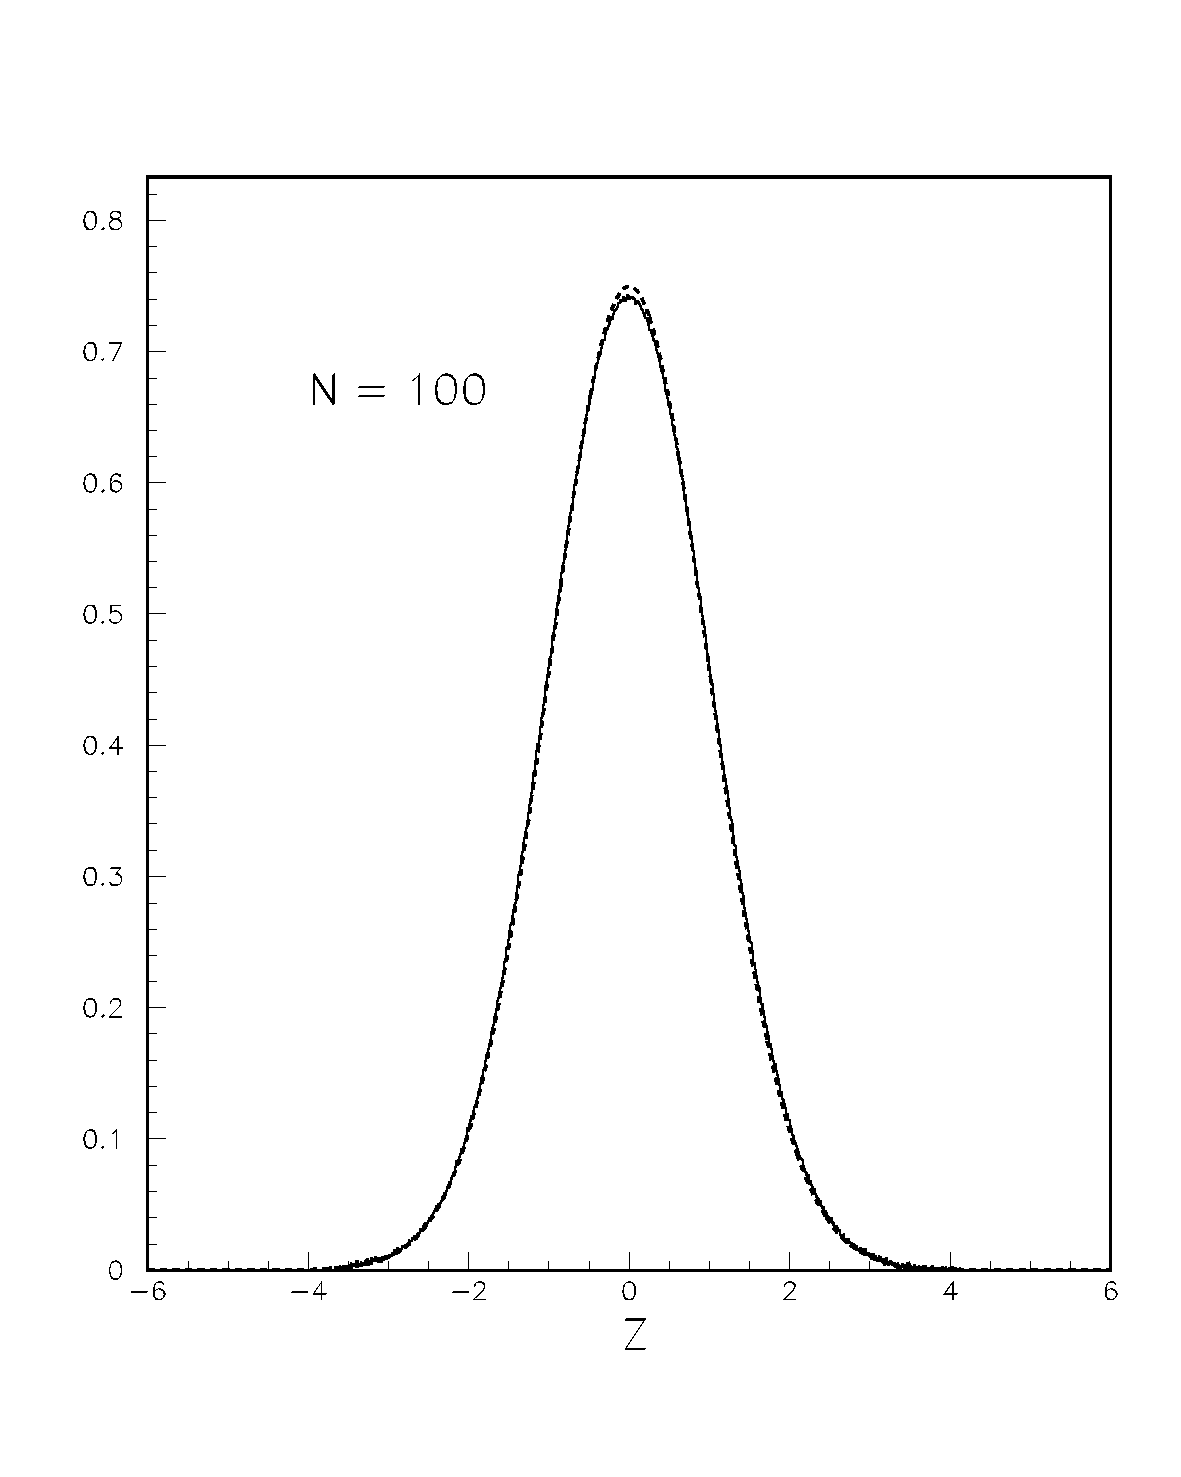
\includegraphics[height=2in,width=2in]{fig3new.pdf}
  \caption{The ground-state wave function for the  
           parameter value $N=mc^2/\hbar\omega=100$ (the non-relativistic
           region) as calculated by the 
           path integral method in Euclidean spacetime (solid) and also
           from the Klein-Gordon Equation (dashed).
           }
\end{center}
\end{figure}

\begin{figure}[htbp]
  \epsfysize=4.0in
  \epsfxsize=6.0in
  \epsfbox{fig3new.eps}
%  \caption{The ground-state wave function for the  
%           parameter value $N=mc^2/\hbar\omega=100$ (the non-relativistic
%           region) as calculated by the 
%           path integral method in Euclidean spacetime (solid) and also
%           from the Klein-Gordon Equation (dashed).
%           }
  \label{fig:nonrel}
\end{figure}
%Figure \ref{fig:compare} 
\begin{figure}[htbp]
  \epsfysize=4.0in
  \epsfxsize=6.0in
  \epsfbox{fig1new.eps}
%  \caption{The ground-state wave function for the  
%           parameter value $N=mc^2/\hbar\omega=1$ as calculated by the 
%           path integral method in Euclidean spacetime (solid) and also
%           from the Klein-Gordon Equation (dashed).
%           }
  \label{fig:compare}
\end{figure}
%Figure \ref{fig:extreme} 
\begin{figure}[htbp]
  \epsfysize=4.0in
  \epsfxsize=6.0in
  \epsfbox{fig2new.eps}
%  \caption{The ground-state wave functions in the relativistic 
%           region at $N=0.01$. The Klein-Gordon theory does not
%           produce a square-integrable ground-state wave function 
%           for $N<1/2$ and is not shown. 
%           Instead we present the best fit of the 
%           Monte Carlo result (solid) to a single Gaussian function 
%           (dashed). Note the non-Gaussian
%           features of the Monte Carlo distribution.
%           }
  \label{fig:extreme}
\end{figure}

\end{document}
%--------------------------------------
% hbar*omega/mc**2 = 100
%   counter =    19990.00
%  <alpha> =  -0.6750870
%  <beta > =    4.331321
%  <gamma> =    8.875617
%--------------------------------------
% hbar*omega/mc**2 = 1
%  counter =    19990.00
%  <alpha> =   0.6034691
%  <beta > =   0.9954181
%  <gamma> =    1.198319
%--------------------------------------
